\begin{frame}{Feature statistics similarity (1/4)}{Anchor age 30}
	\begin{tikzpicture}[remember picture, overlay]
		\node[right=0.28\textwidth,below=4.5em] at (current page.north west) 
		{
			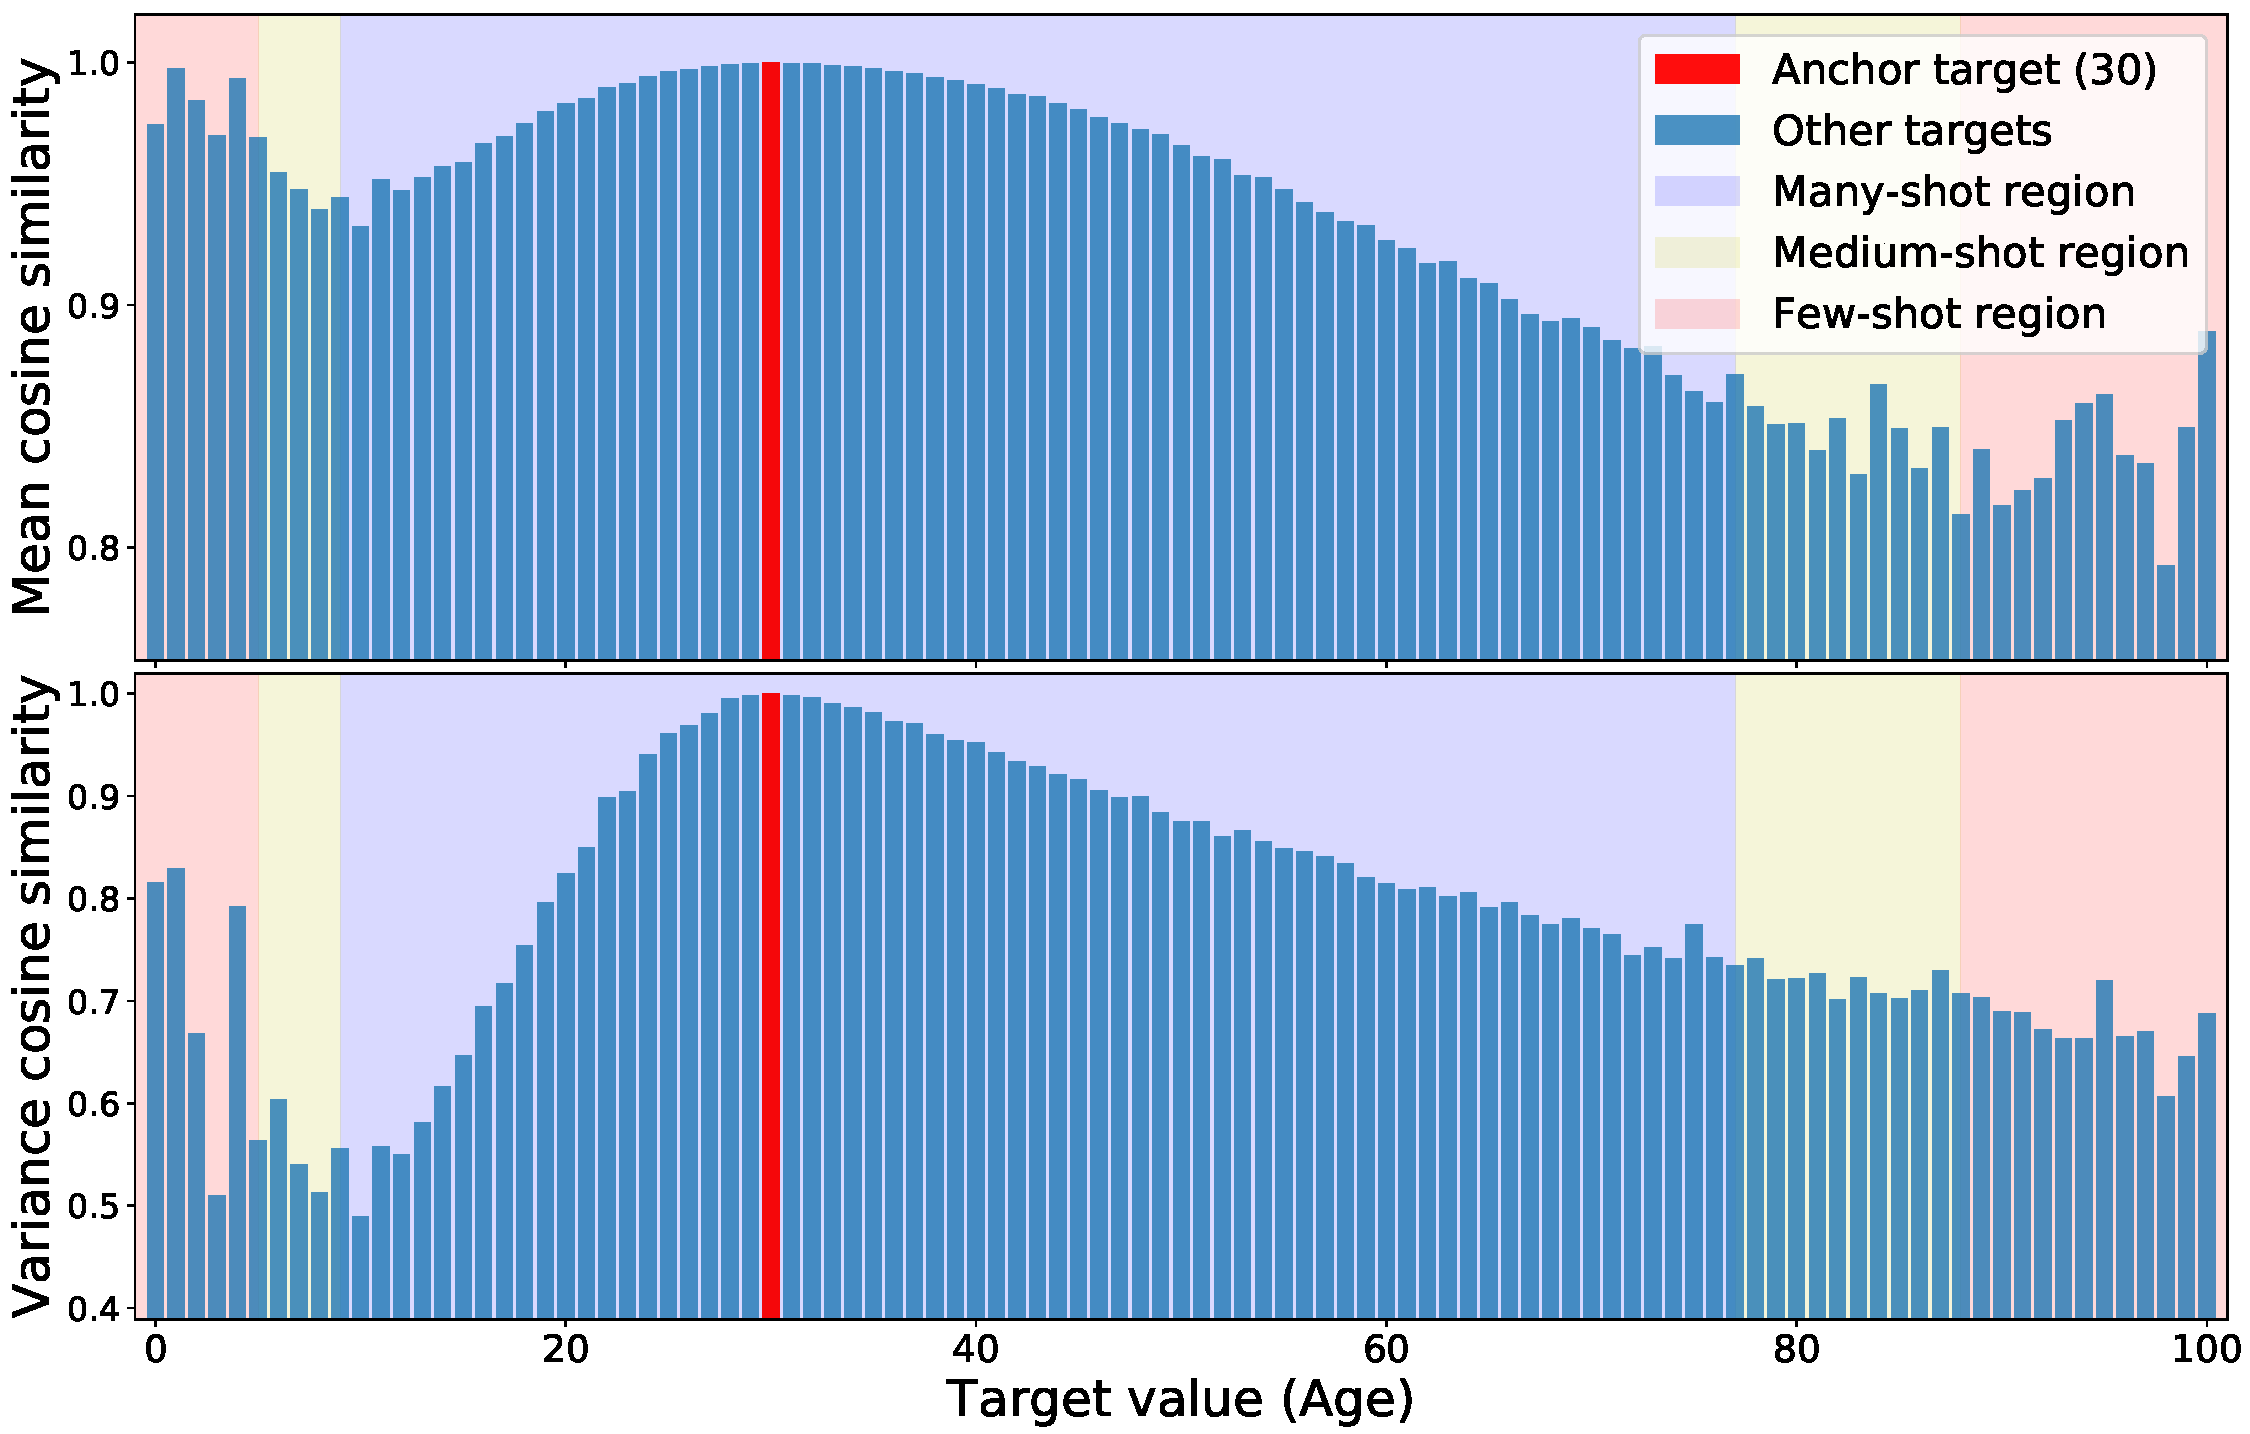
\includegraphics[width=0.5\textwidth]{images/feat_sim_fds_base_30.pdf}
		};
		\node[left=0.27\textwidth,below=4.5em] at (current page.north east) 
		{
			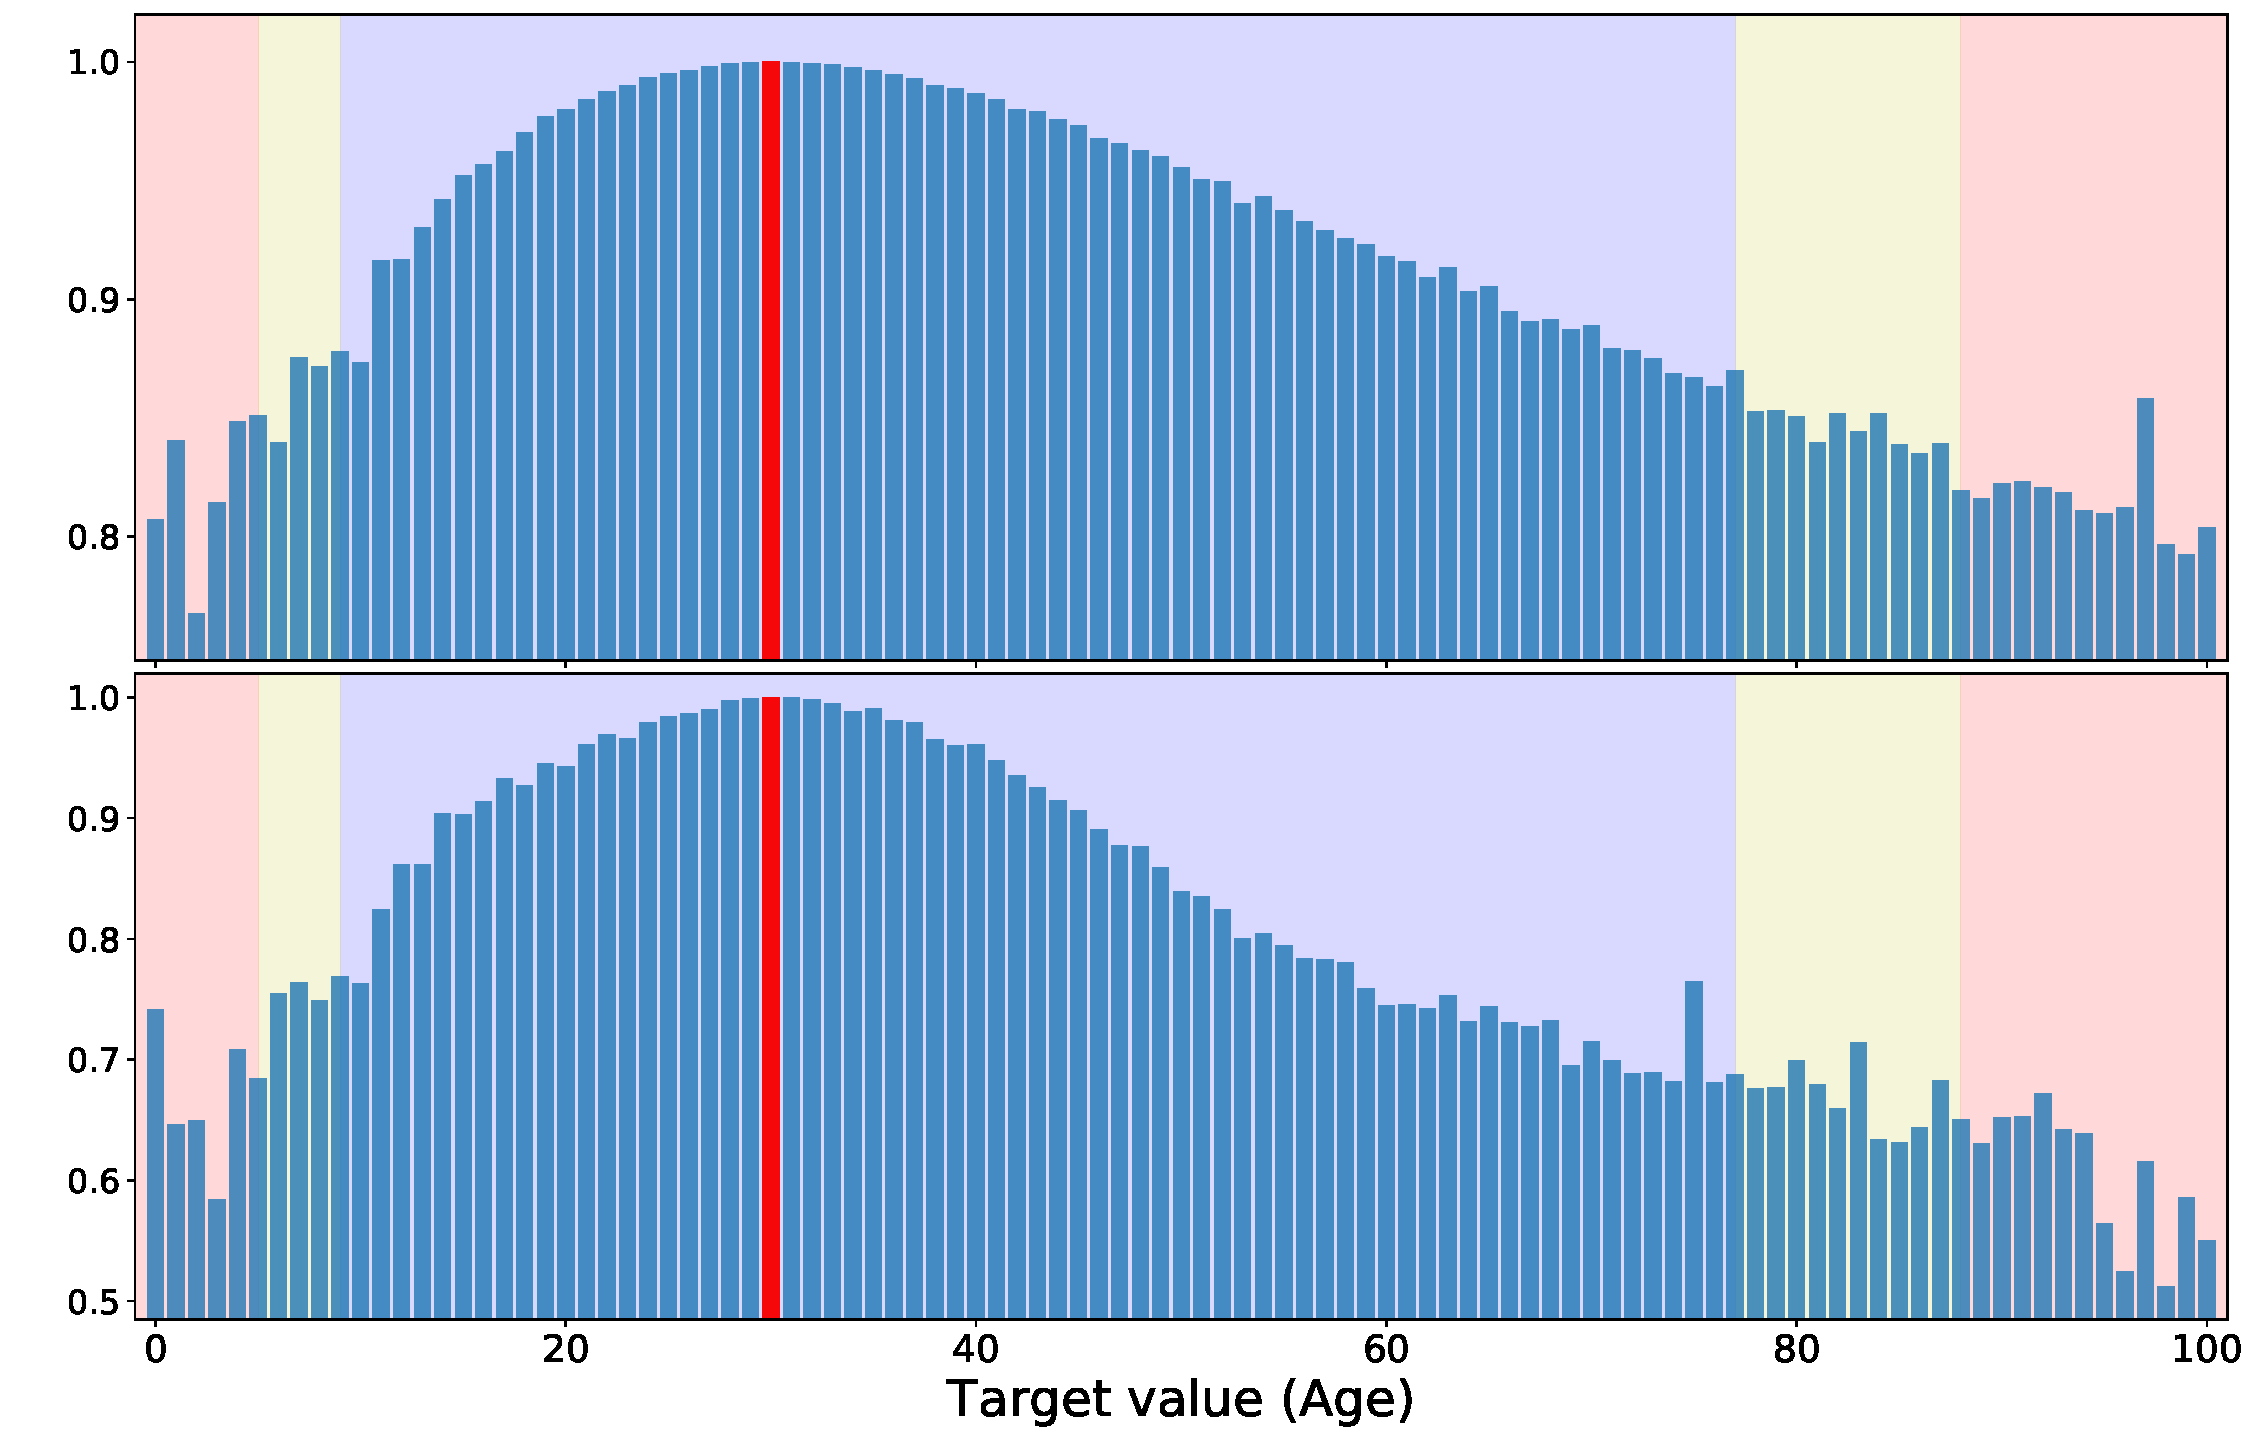
\includegraphics[width=0.49\textwidth]{images/feat_sim_fds_ours_30.pdf}
		};
	\end{tikzpicture}
	\vspace{0.45\textheight}
	\begin{columns}[T]
		\footnotesize
		\begin{column}{0.5\textwidth}
			\begin{itemize}
				\item High similarity in neighbourhood
				\item \red{High similarities with further regions}
				\item \red{Lower similarities with some closer regions}
			\end{itemize}
		\end{column}
		\begin{column}{0.5\textwidth}
			\begin{itemize}
				\item Improved feature statistics calibration:
				\begin{itemize}
					\vspace{-1.5em}
					\scriptsize
					\item High similarity only in neighbourhood
					\item ``The further the region the lower the similarity''
					\item More gradual similarity change
				\end{itemize}
			\end{itemize}
		\end{column}
	\end{columns}
	\credit{Image}{yang2021delving}
\end{frame}

\begin{frame}{Feature statistics similarity (2/4)}{Anchor age 60}
	\begin{tikzpicture}[remember picture, overlay]
		\node[right=0.28\textwidth,below=4.5em] at (current page.north west) 
		{
			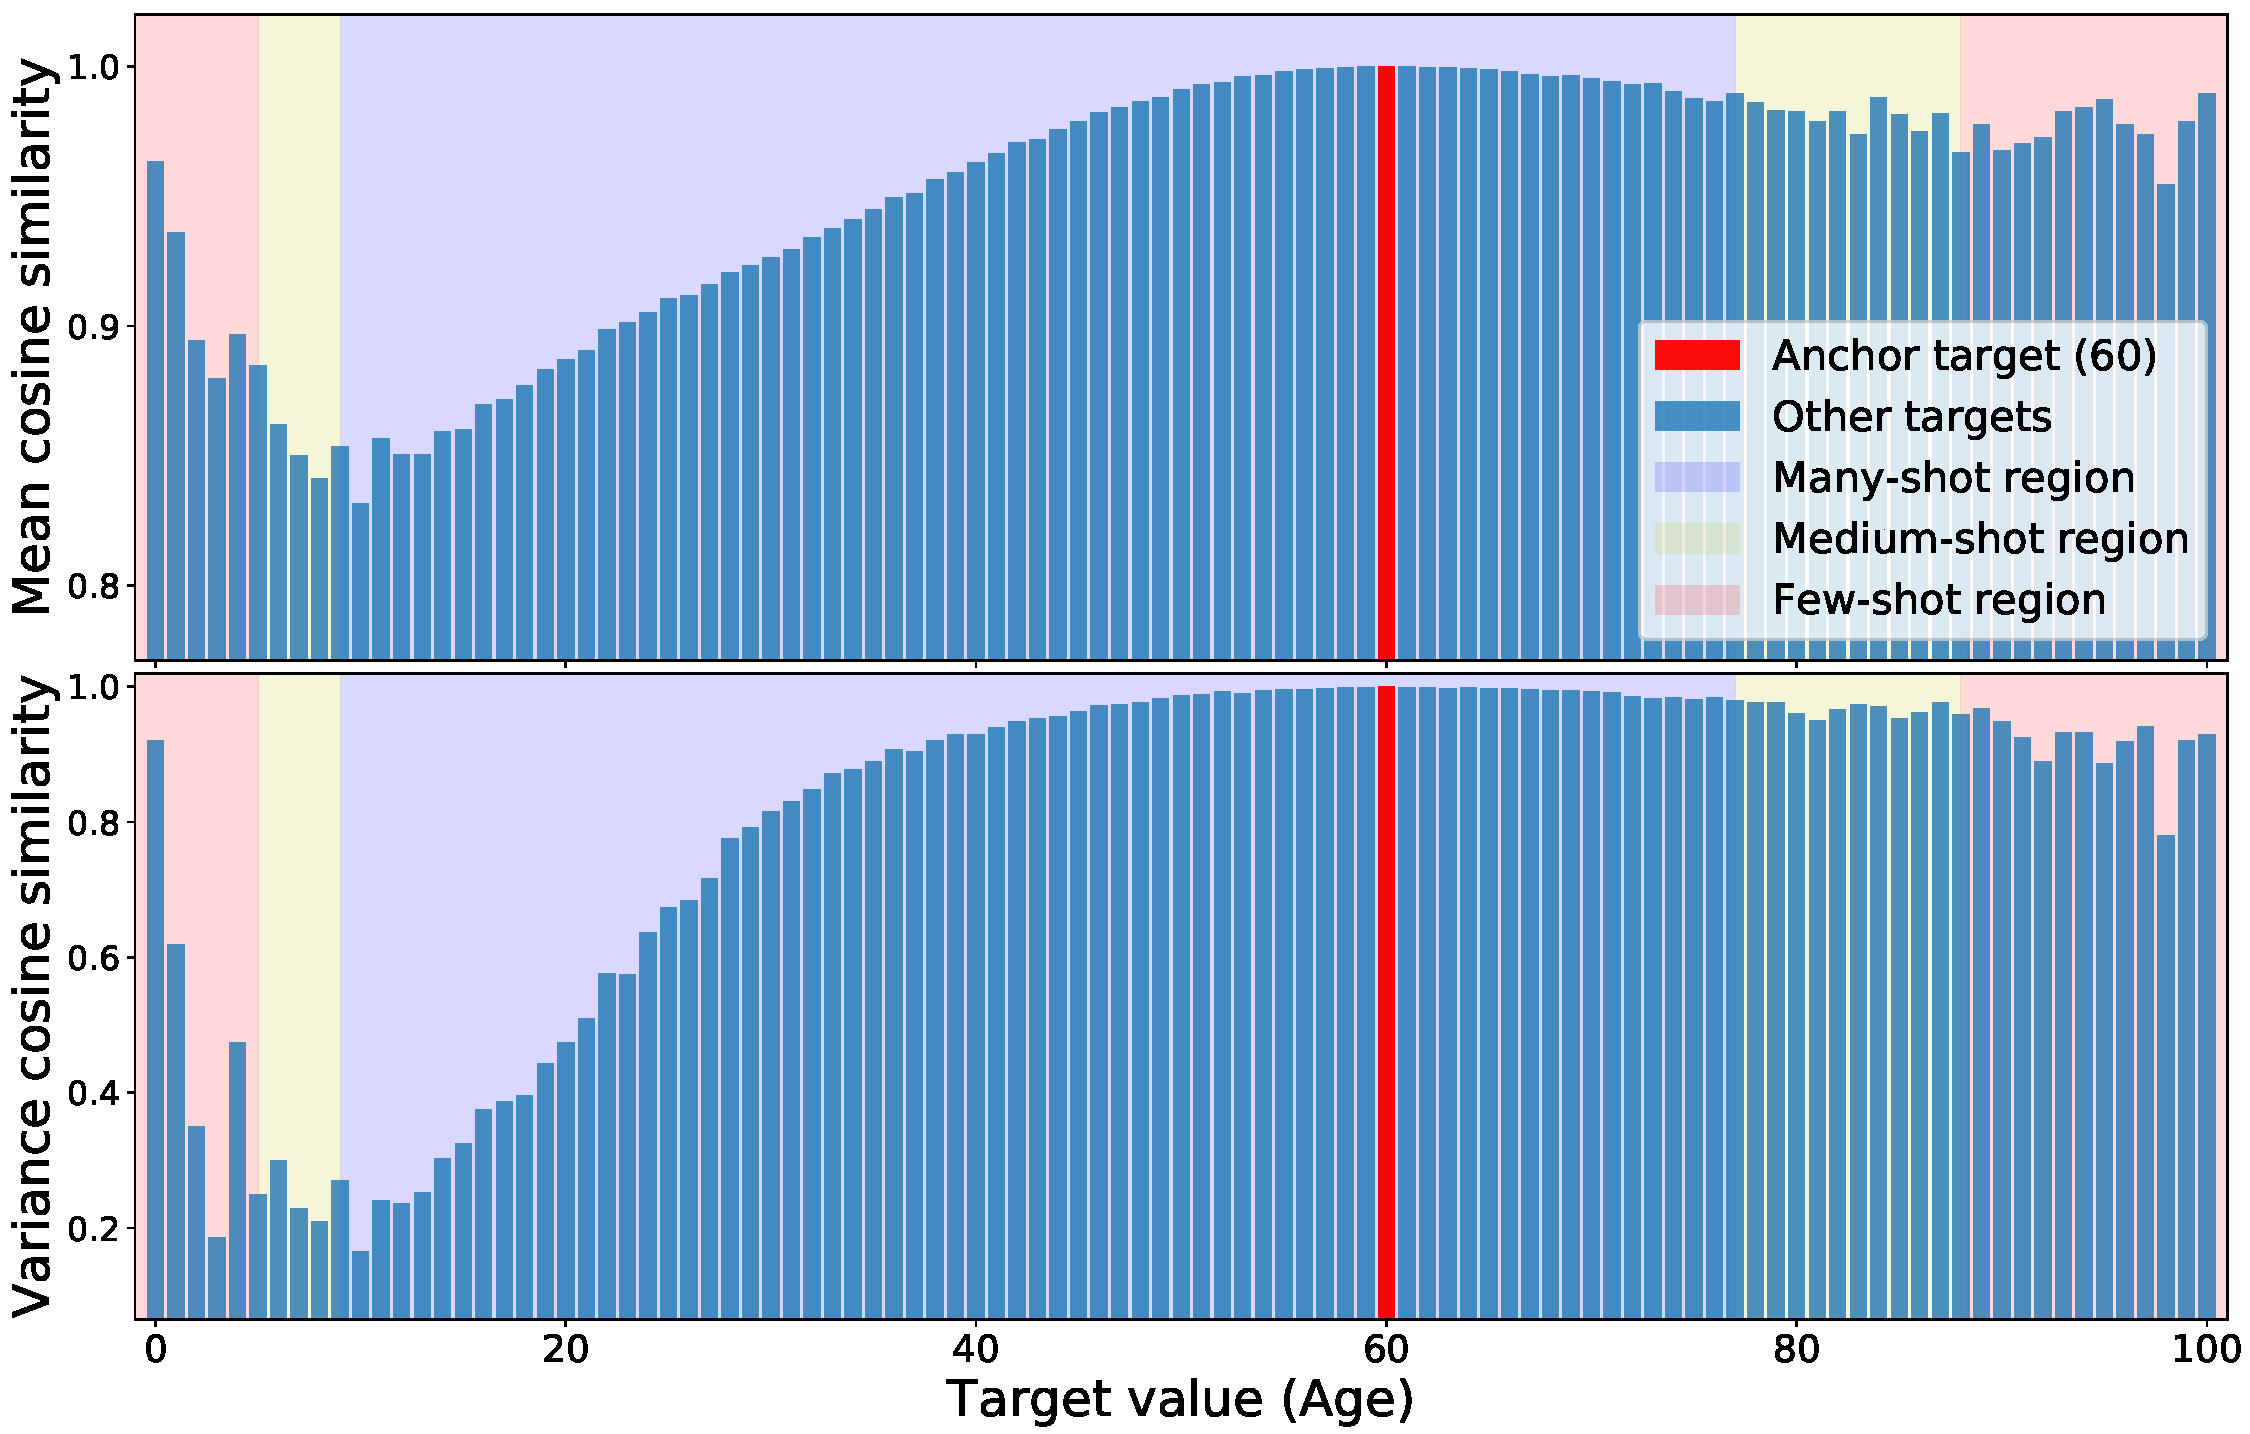
\includegraphics[width=0.5\textwidth]{images/feat_sim_fds_base_60.pdf}
		};
		\node[left=0.27\textwidth,below=4.5em] at (current page.north east) 
		{
			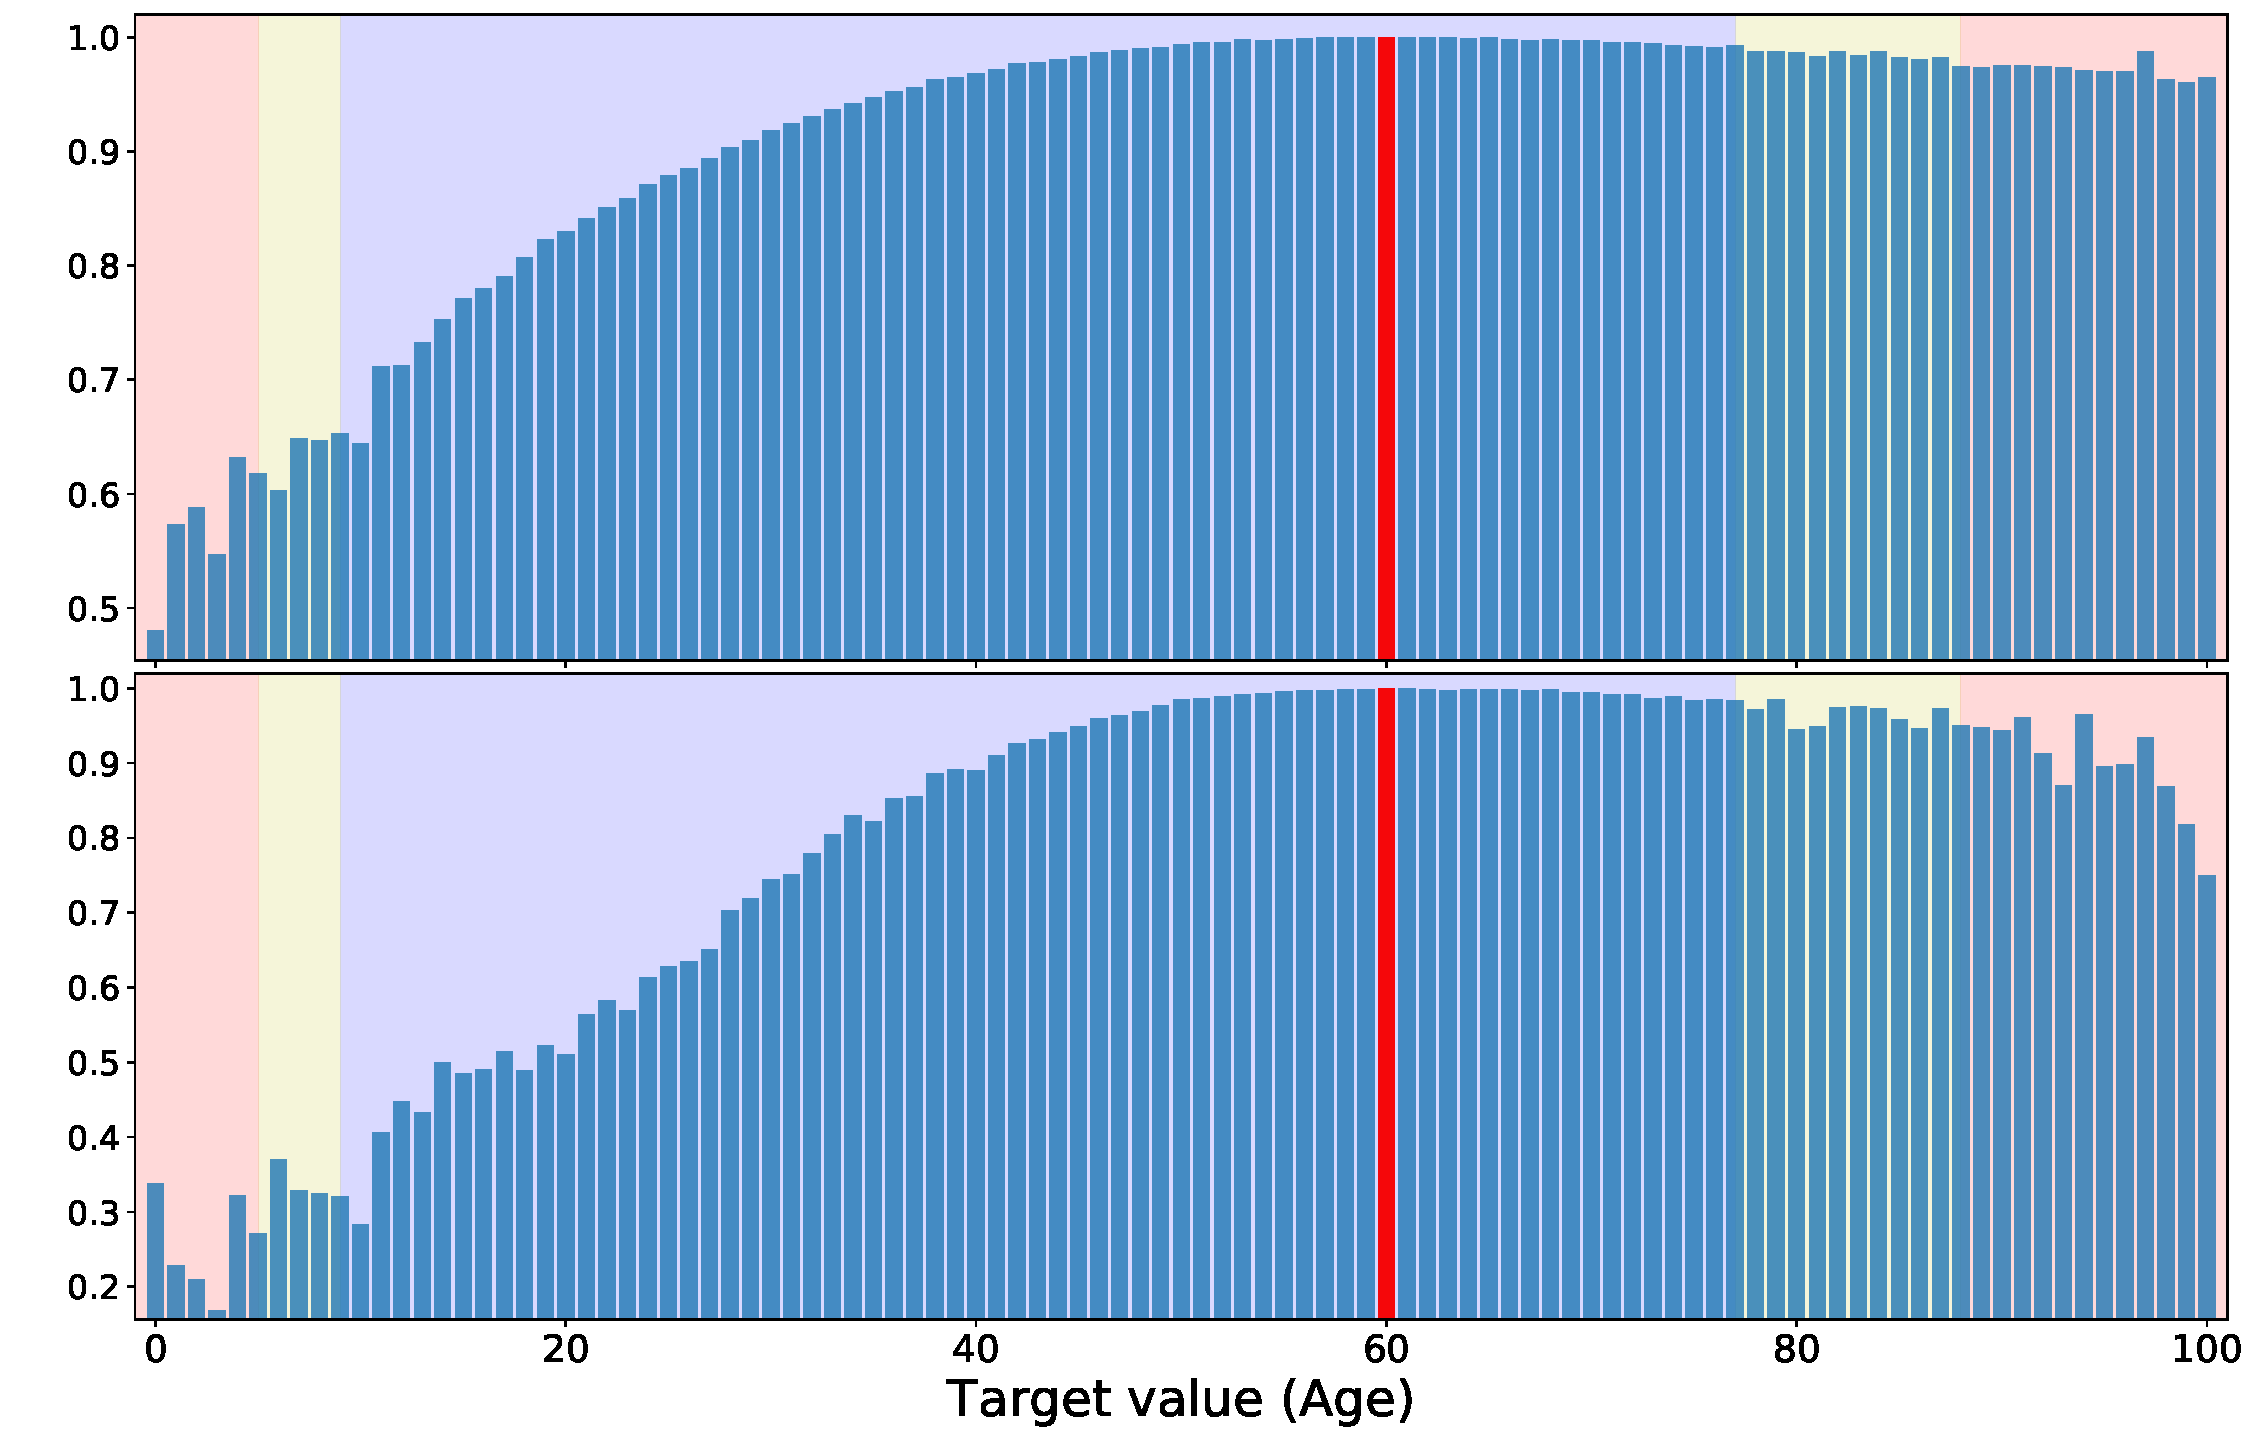
\includegraphics[width=0.49\textwidth]{images/feat_sim_fds_ours_60.pdf}
		};
	\end{tikzpicture}
	\vspace{0.45\textheight}
	\begin{columns}[T]
		\footnotesize
		\begin{column}{0.5\textwidth}
			\begin{itemize}
				\item High similarity in neighbourhood
				\item \red{High similarities with further regions}
				\item \red{Lower similarities with some closer regions}
			\end{itemize}
		\end{column}
		\begin{column}{0.5\textwidth}
			\begin{itemize}
				\item Improved feature statistics calibration:
				\begin{itemize}
					\vspace{-1.5em}
					\scriptsize
					\item High similarity only in neighbourhood
					\item ``The further the region the lower the similarity''
					\item More gradual similarity change
				\end{itemize}
			\end{itemize}
		\end{column}
	\end{columns}
	\credit{Image}{yang2021delving}
\end{frame}

\begin{frame}{Feature statistics similarity (3/4)}{Anchor age 0}
	\begin{tikzpicture}[remember picture, overlay]
		\node[right=0.28\textwidth,below=4.5em] at (current page.north west) 
		{
			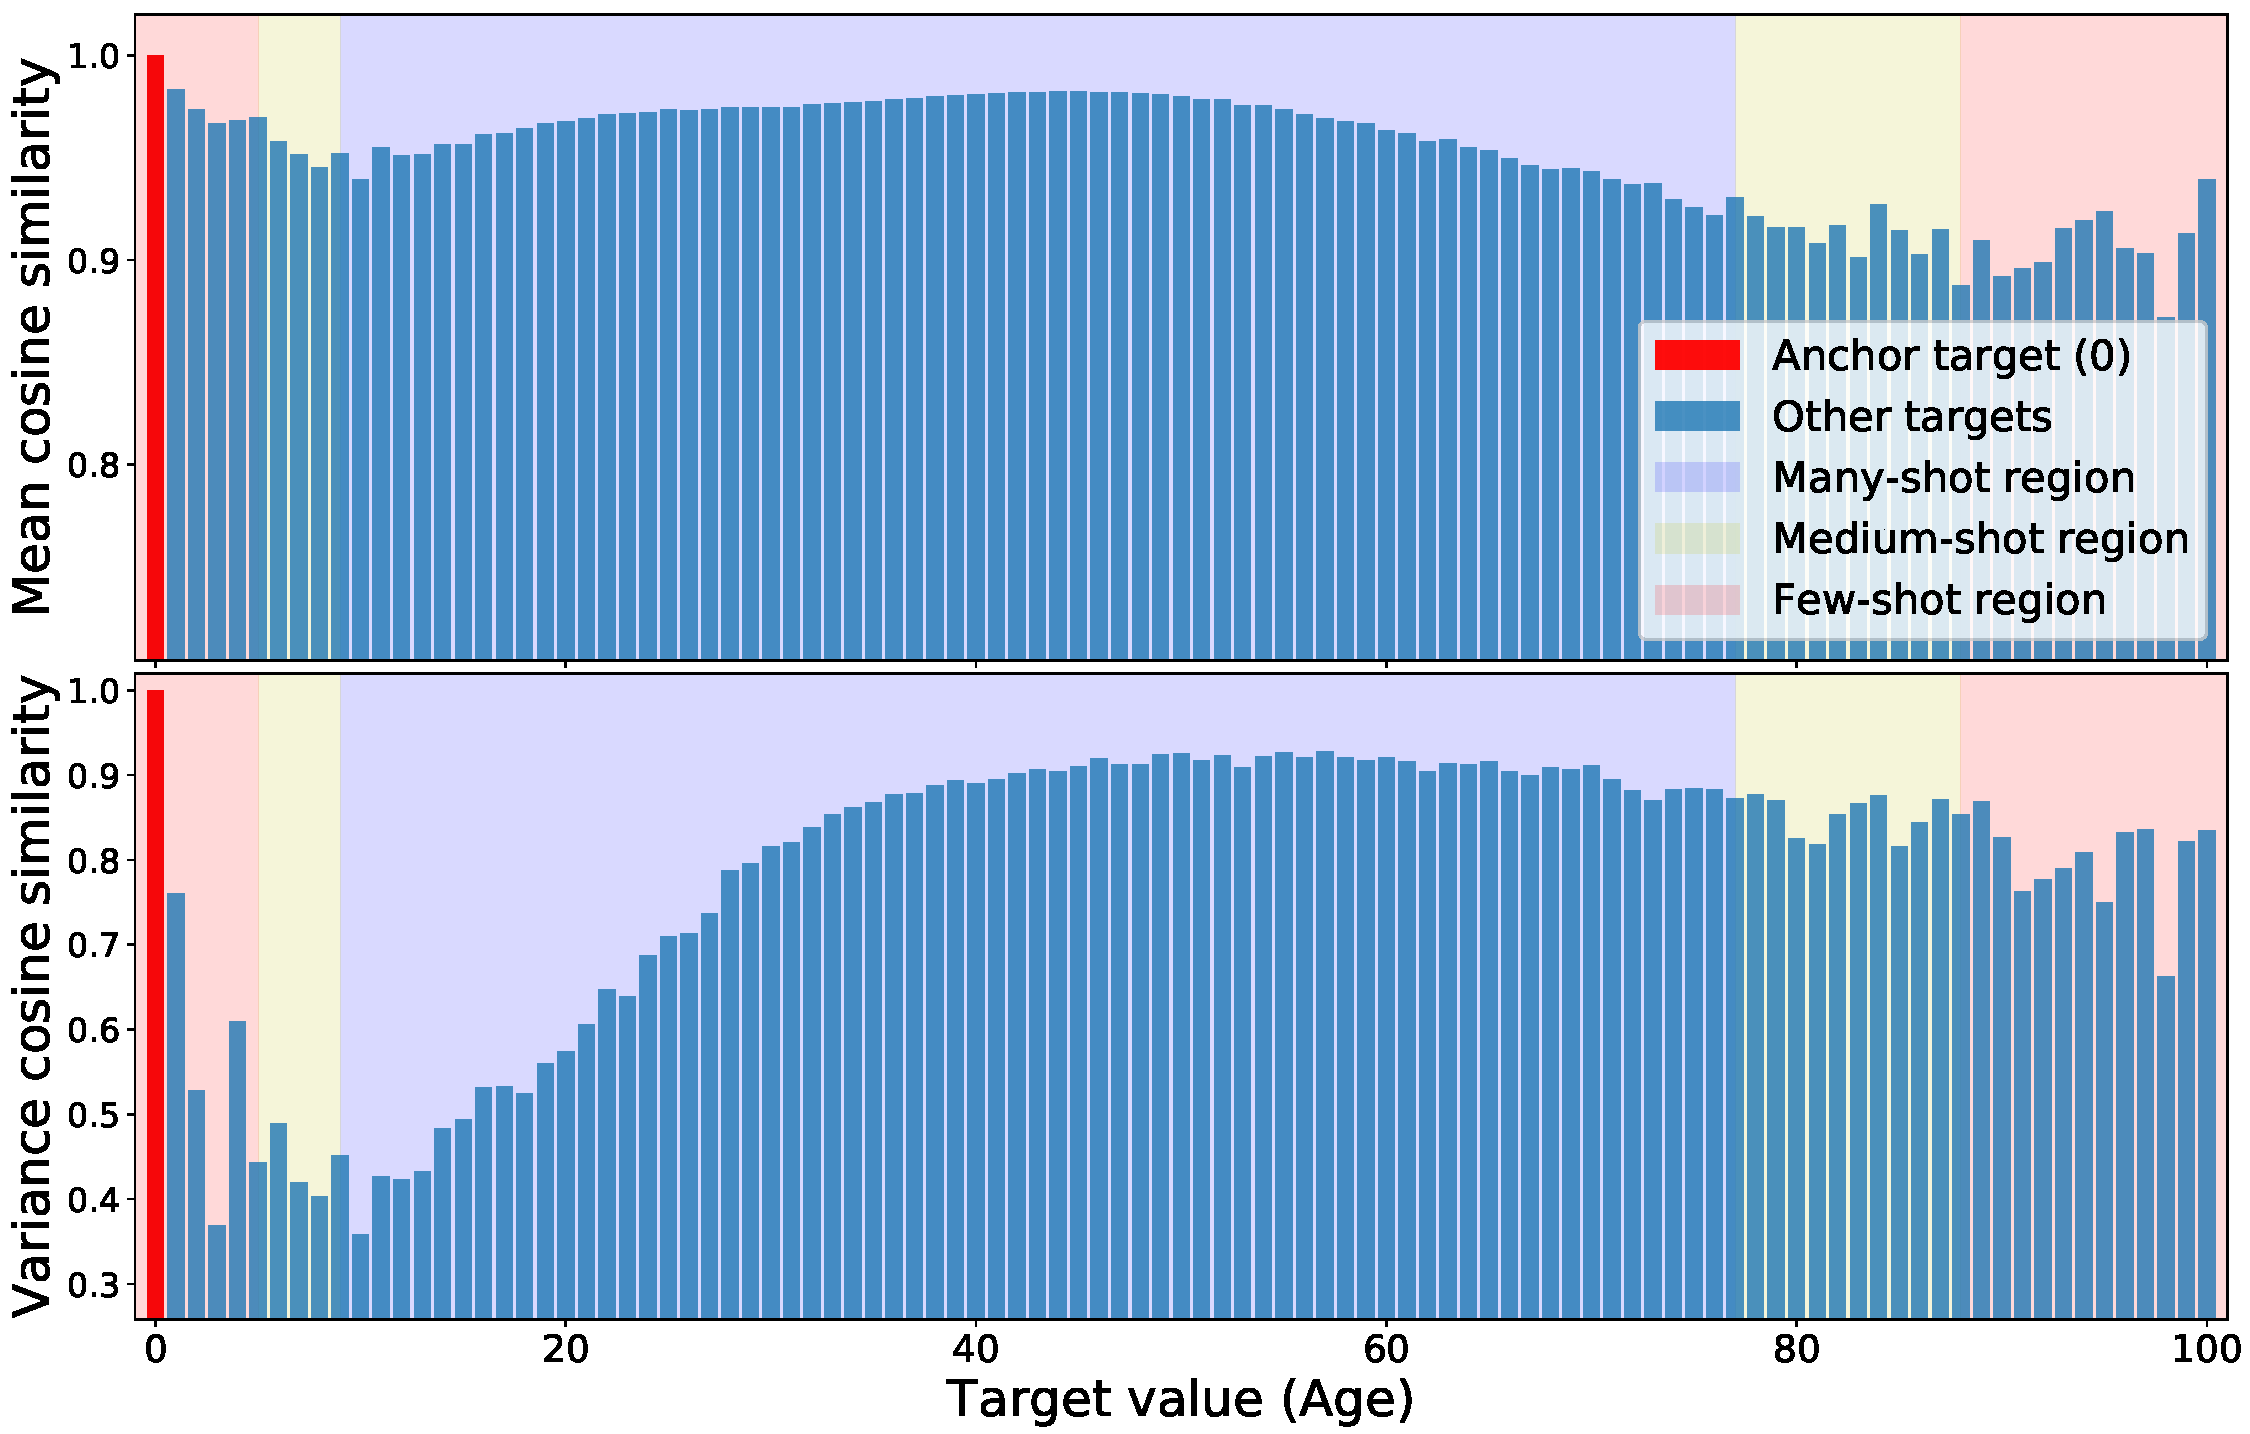
\includegraphics[width=0.5\textwidth]{images/feat_sim_fds_base_0.pdf}
		};
		\node[left=0.27\textwidth,below=4.5em] at (current page.north east) 
		{
			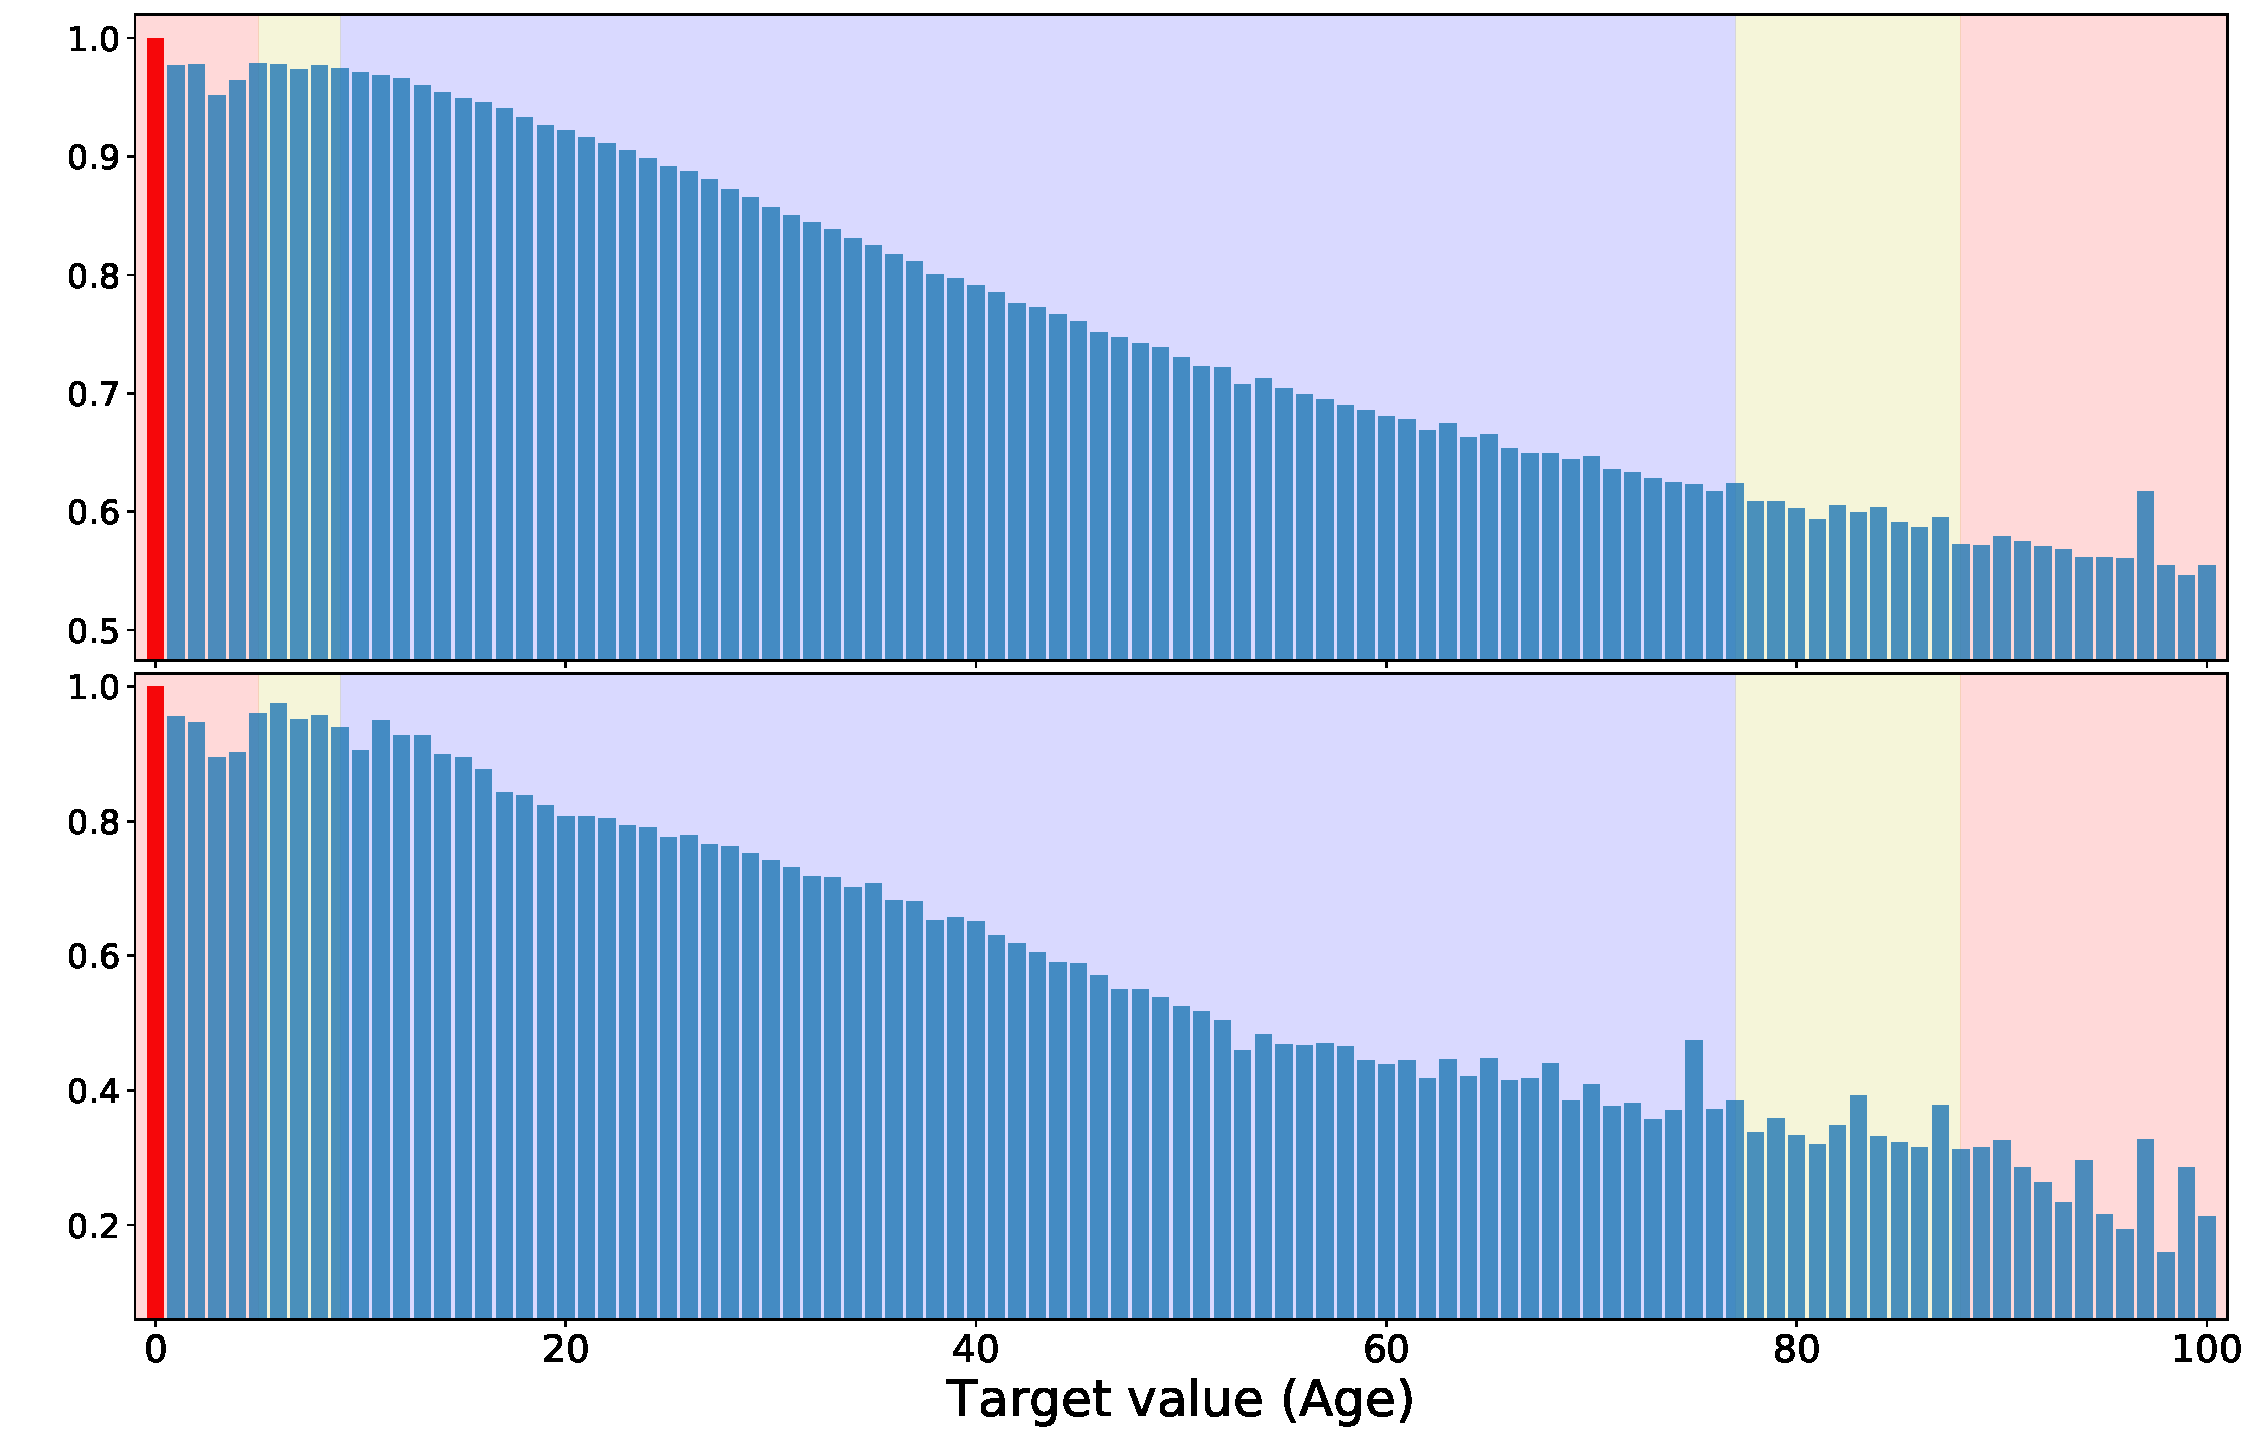
\includegraphics[width=0.49\textwidth]{images/feat_sim_fds_ours_0.pdf}
		};
	\end{tikzpicture}
	\vspace{0.45\textheight}
	\begin{columns}[T]
		\footnotesize
		\begin{column}{0.5\textwidth}
			\begin{itemize}
				\item High similarity in neighbourhood for mean
				\item \red{High similarities with further regions}
				\item \red{Lower similarities with some closer regions, e.g., variance neighbourhood}
			\end{itemize}
		\end{column}
		\begin{column}{0.5\textwidth}
			\begin{itemize}
				\item Improved feature statistics calibration:
				\begin{itemize}
					\vspace{-1.5em}
					\scriptsize
					\item High similarity only in neighbourhood
					\item ``The further the region the lower the similarity''
					\item More gradual similarity change
				\end{itemize}
			\end{itemize}
		\end{column}
	\end{columns}
	\credit{Image}{yang2021delving}
\end{frame}

\begin{frame}{Feature statistics similarity (4/4)}{Anchor age 90}
	\begin{tikzpicture}[remember picture, overlay]
		\node[right=0.28\textwidth,below=4.5em] at (current page.north west) 
		{
			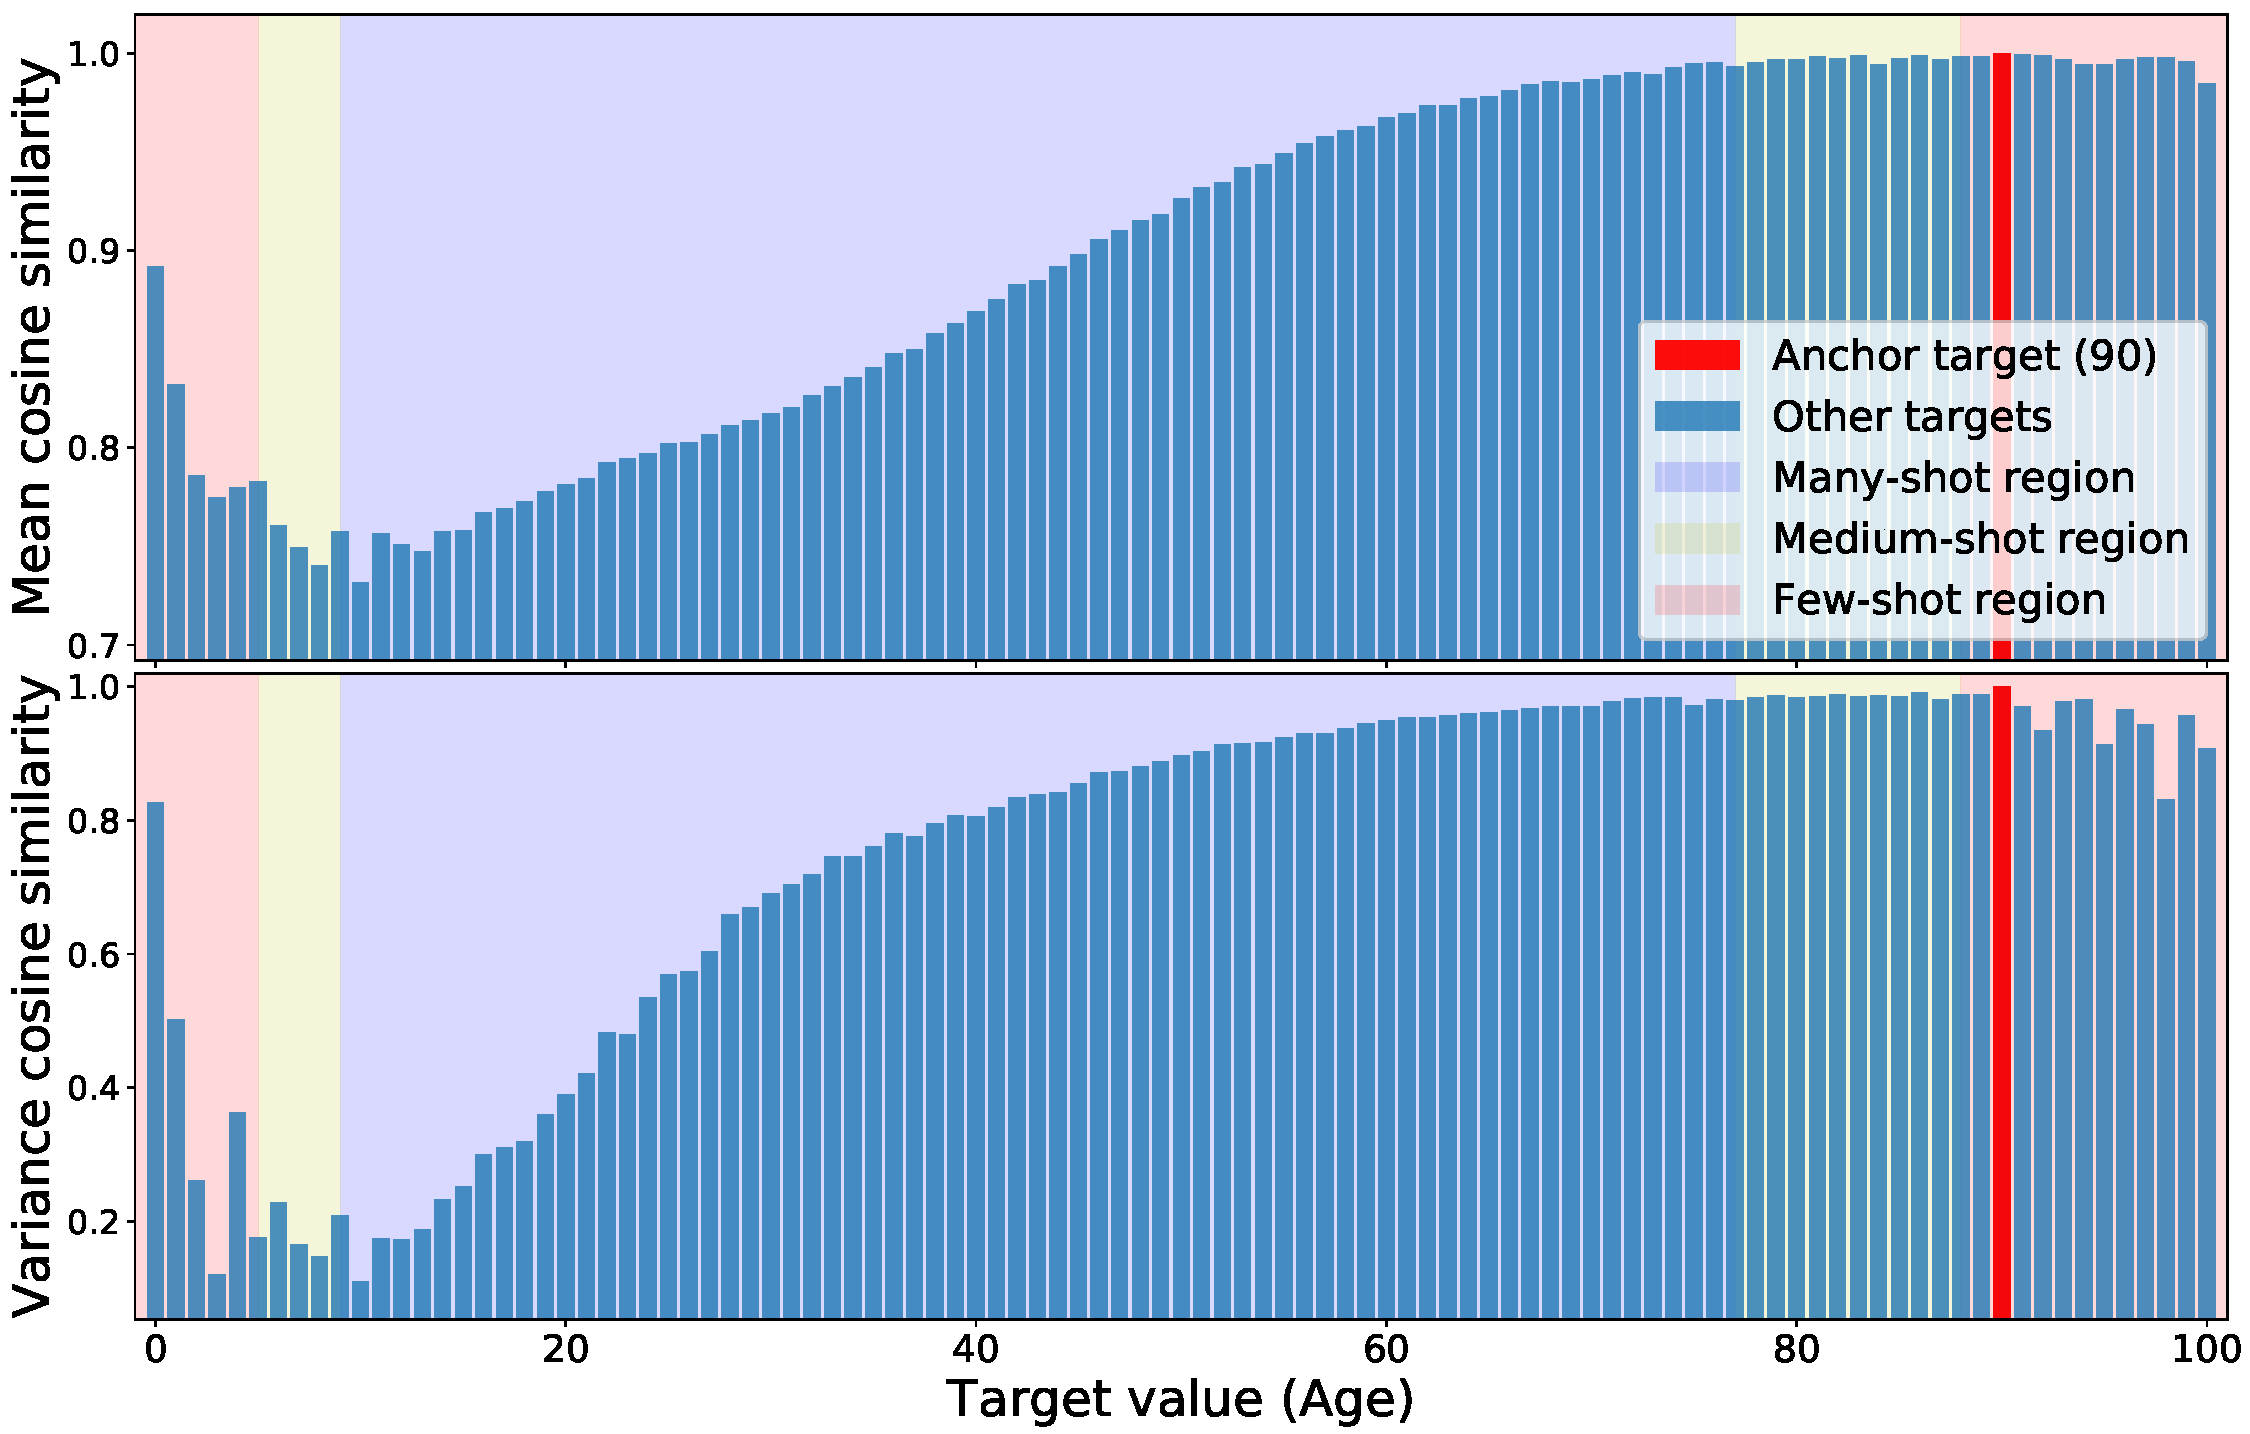
\includegraphics[width=0.5\textwidth]{images/feat_sim_fds_base_90.pdf}
		};
		\node[left=0.27\textwidth,below=4.5em] at (current page.north east) 
		{
			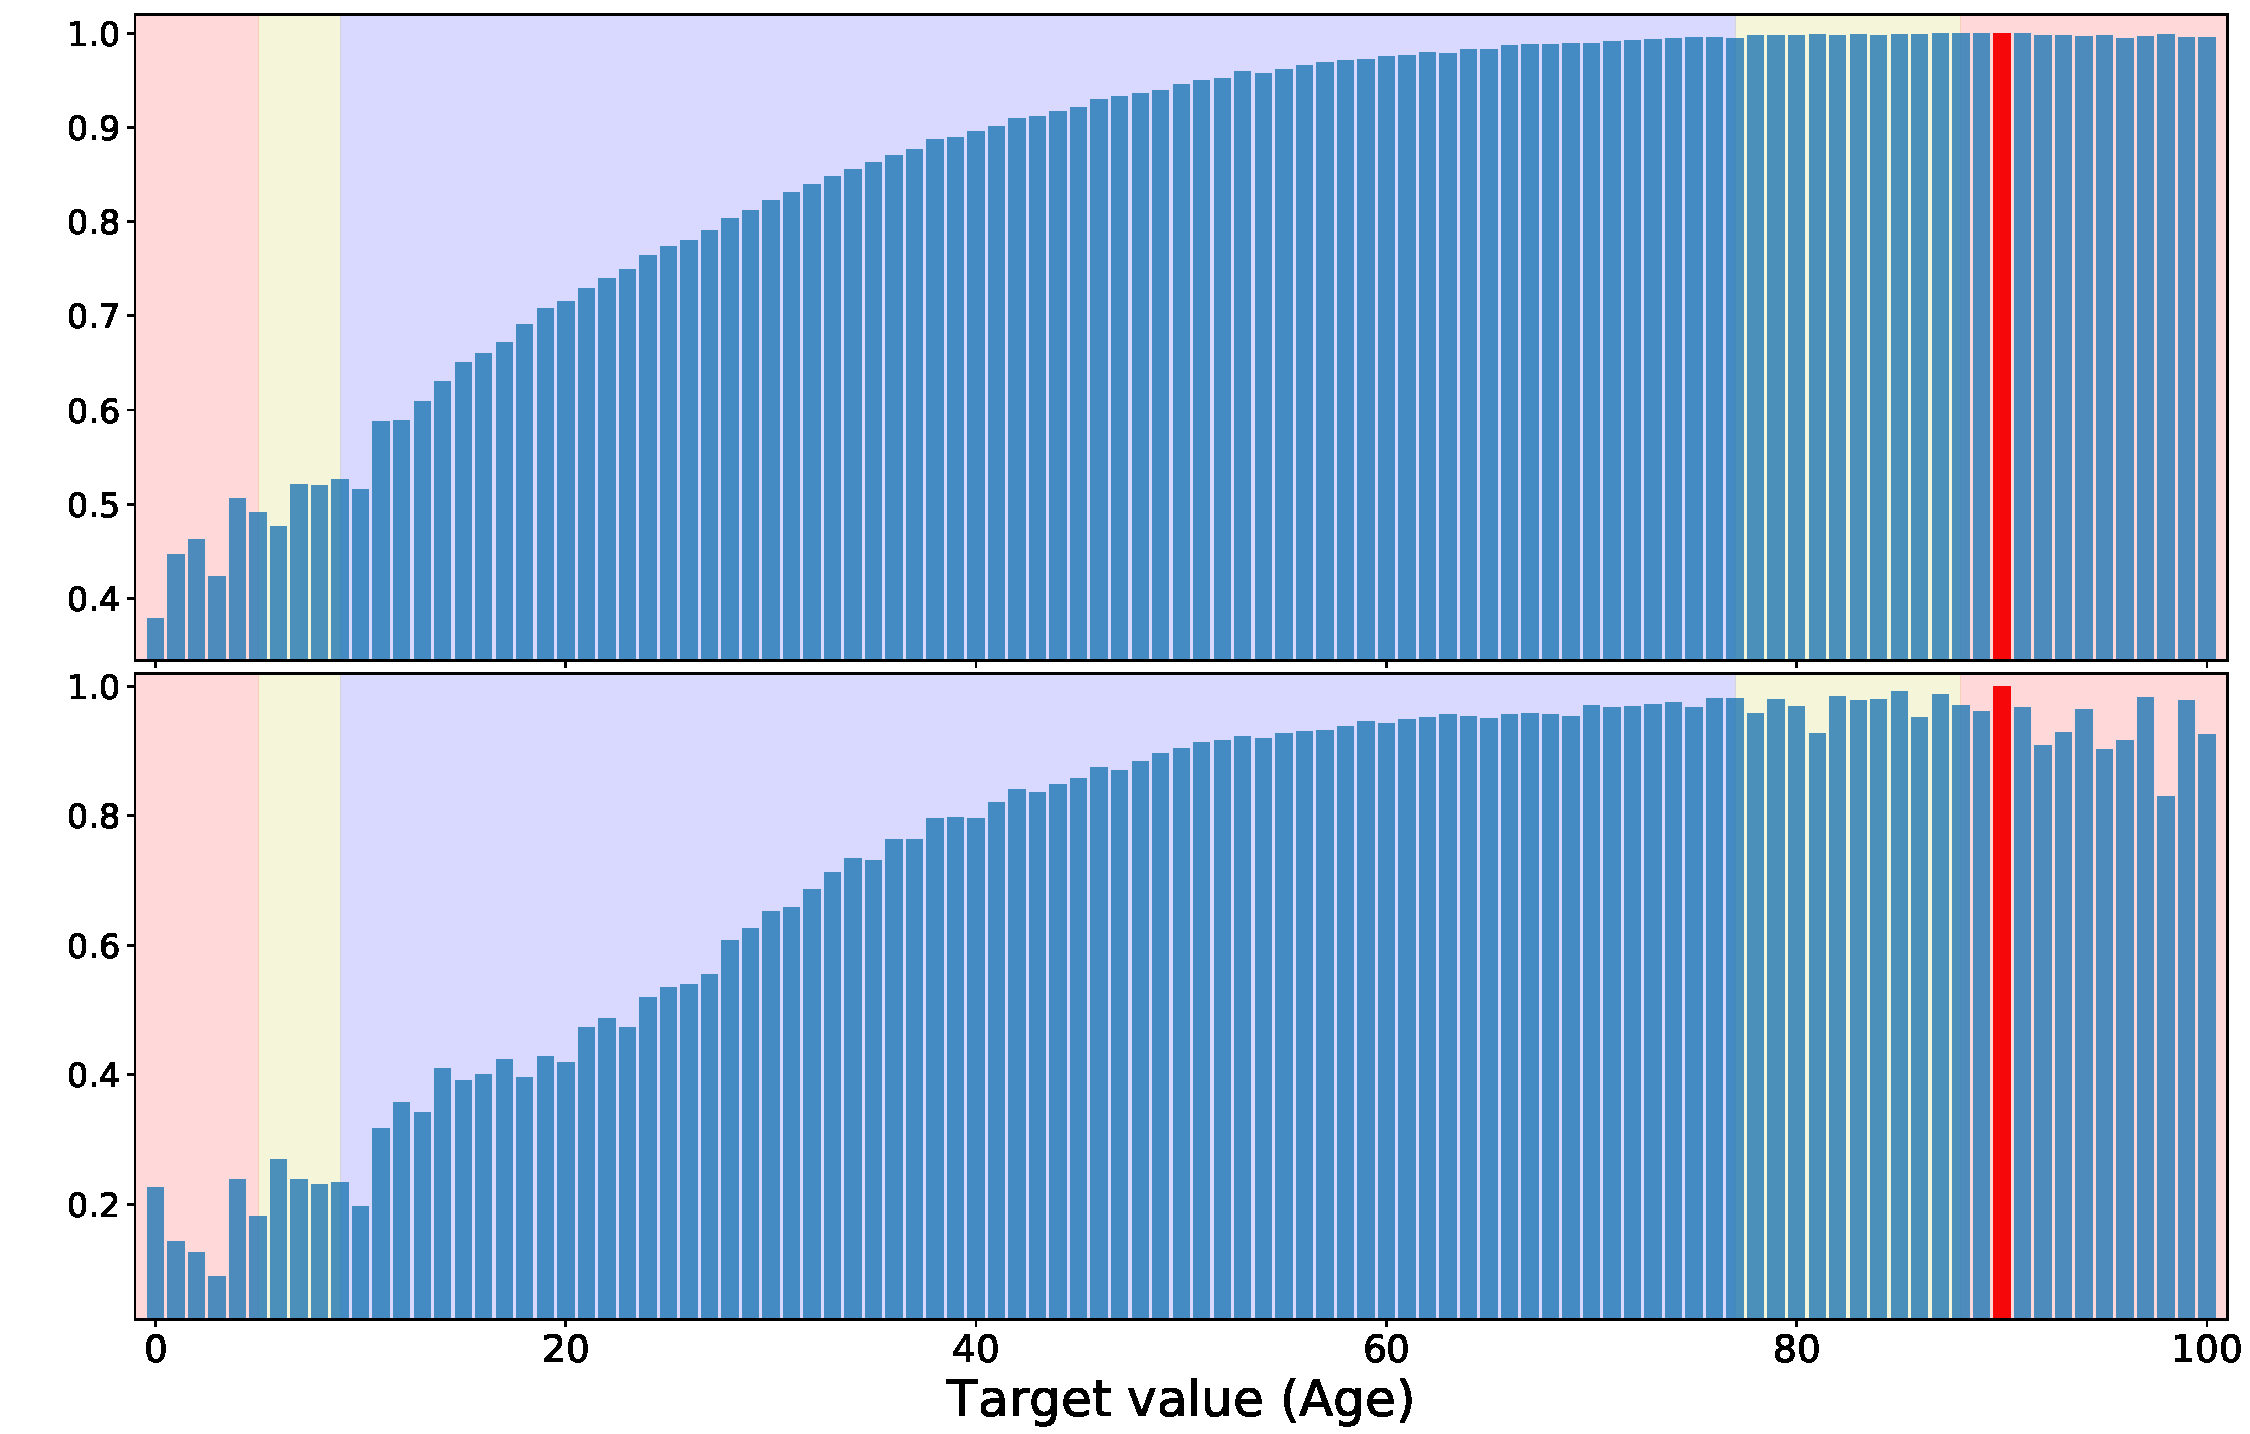
\includegraphics[width=0.49\textwidth]{images/feat_sim_fds_ours_90.pdf}
		};
	\end{tikzpicture}
	\vspace{0.45\textheight}
	\begin{columns}[T]
		\footnotesize
		\begin{column}{0.5\textwidth}
			\begin{itemize}
				\item High similarity in neighbourhood, \\esp. for mean
				\item \red{High similarities with further regions}
				\item \red{Lower similarities with some closer regions}
			\end{itemize}
		\end{column}
		\begin{column}{0.5\textwidth}
			\begin{itemize}
				\item Improved feature statistics calibration:
				\begin{itemize}
					\vspace{-1.5em}
					\scriptsize
					\item High similarity only in neighbourhood
					\item ``The further the region the lower the similarity''
					\item More gradual similarity change
				\end{itemize}
			\end{itemize}
		\end{column}
	\end{columns}
	\credit{Image}{yang2021delving}
\end{frame}